
Folgende Abbildung zeigt eine grundlegende Übersicht der wichtigsten Klassen und deren Zusammenwirken.
\begin{center}
    \begin{figure}[H]
        \centering
        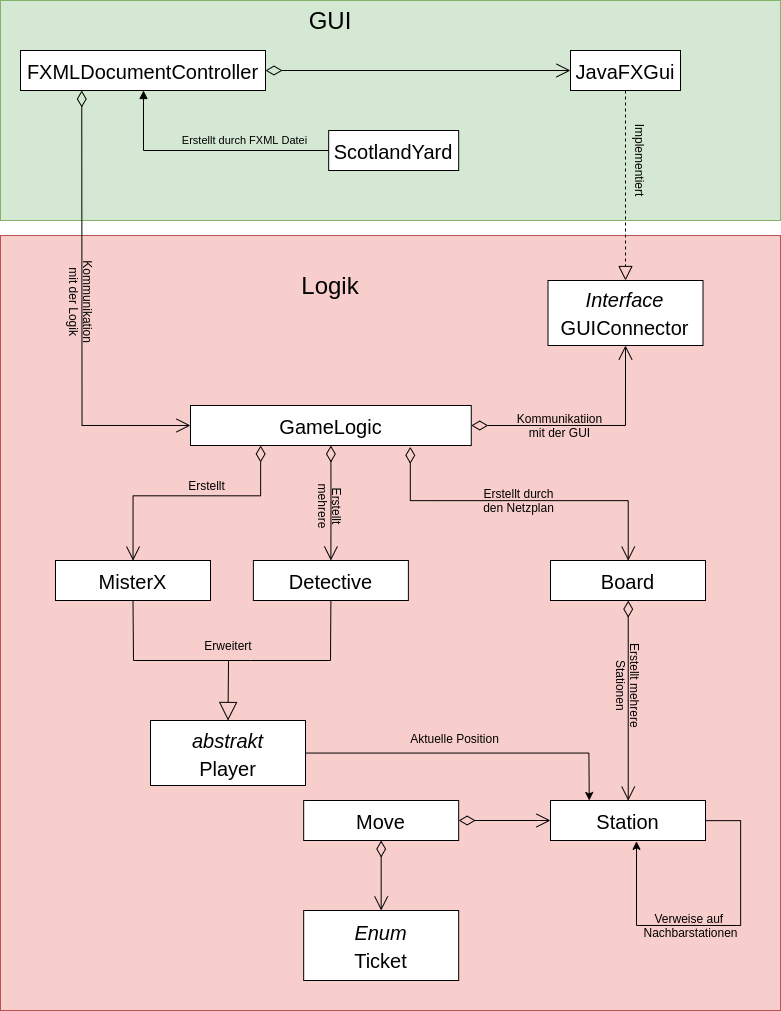
\includegraphics[scale=0.35]{img/uml/pop.png}   
        \caption{Vereinfachter Programmorganisationsplan}
    \end{figure}
\end{center}
Beim Programmstart wird die \textit{main}-Methode innerhalb der \textit{ScotlandYard}-Klasse ausgeführt.
Da die \textit{ScotlandYard}-Klasse die \textit{Application}-Klasse erweitert, wird beim aufrufen ihrer \textit{start}-Methode
die FXML-Datei geladen und daraus der \textit{FXMLDocumentController} erstellt.
Der \textit{FXMLDocumentController} besitzt alle graphischen Elemente der Oberfläche und erstellt daraus die \textit{JavaFXGui}-Klasse
und übergibt diese beim erstellen an die \textit{GameLogic}.
\newline
\newline
Die \textit{GameLogic} erstellt durch die Parameter ihres Konstruktors jeweils \textit{MisterX}, mehrere Instanzen von \textit{Detective}
und das Spielfeld (\textit{Board}). \textit{MisterX} und \textit{Detective} sind dabei Speziallisierungen der abstrakten \textit{Player}-Klasse.
Durch die übergebene \textit{JavaFXGui}-Instanz, die den \textit{GUIConnector} implementiert, kann die \textit{GameLogic} die GUI direkt manipulieren.
\newline
\newline
Das \textit{Board} erstellt beim Instanziieren alle nötigen Stationen die jeweils Referenzen auf ihre Nachbarstationen halten.